\chapter{Ход работы}

\textbf{Цель работы}: провести модельное исследование неинвертирующего усилителя с использованием выбранных элементов.

Исходные данные: условия (дано) из ДЗ и результаты расчетов

\begin{figure}[h!]
	\centering
	\caption{– Схема неинвертирующего усилителя}
	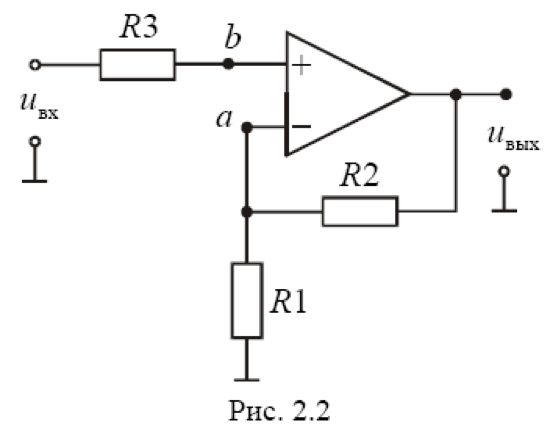
\includegraphics{images/1.png}
\end{figure}


\begin{figure}[h!]
	\centering
	\caption{Модель системы в OrCAD Capture}
	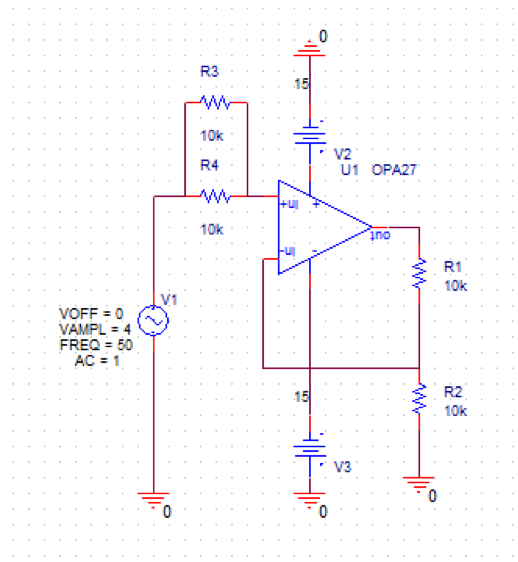
\includegraphics{images/2.png}
\end{figure}

\chapter{Результаты моделирования}

\begin{figure}[h!]
	\centering
	\caption{Входное напряжение (зеленый, В), выходное напряжение (красный, В) }
	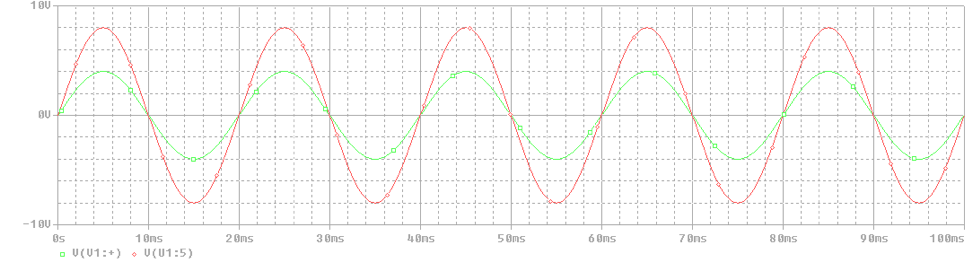
\includegraphics{images/3.png}
\end{figure}

\begin{figure}[h!]
	\centering
	\caption{Выходное напряжение (красный, В), максимальное выходное напряжение (фиолетовый, В), минимальное выходное напряжение (синий, В)}
	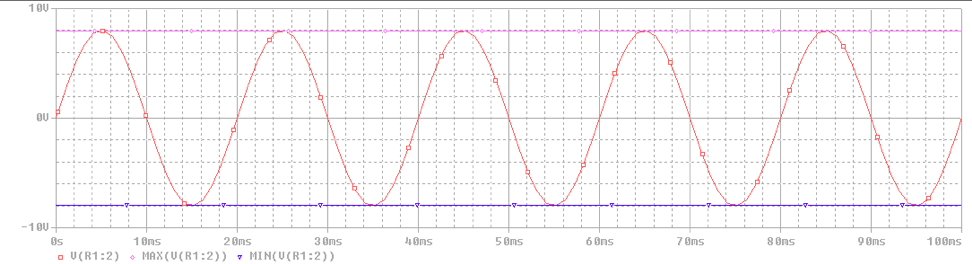
\includegraphics{images/4.png}
\end{figure}

\begin{figure}[h!]
	\centering
	\caption{АЧХ}
	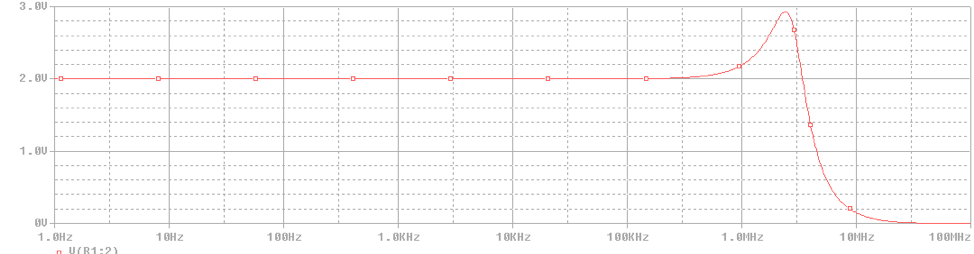
\includegraphics{images/5.png}
\end{figure}



\chapter{Измерения в OrCAD Capture}

Максимальное выходное напряжение, В:   				          

\[
 U_{OUT\_MAX\_EXP}=7.9839
 \]

Минимальное выходное напряжение, В:

\[
U_{OUT\_MIN\_EXP}=-7.9839
\]

\chapter{Вычисление погрешностей}

Погрешность $U_{OUT\_MAX}$:

\[
\left| \frac{U_{OUT\_MAX\_EXP-U_{OUT\_MAX}}}{U_{OUT\_MAX}}\right|=0,2%
\]


Погрешность $U_{OUT\_MIN}$:
\[
\left| \frac{U_{OUT\_MIN\_EXP}-U_{OUT\_MIN}}{U_{OUT\_MIN}}\right|=0,2 %
\]

\chapter{Вывод}

В ходе выполнения лабораторной работы было был промоделирован неинвертирующий усилитель, построены графики изменения величин в OrCAD PSpice, измерены необходимые величины по этим графикам и рассчитаны погрешности.

Вычисленные погрешности демонтрируют минимальное отклонение от расчетных значений, что свидетельствует о корректности выполнения работы и соответствии модели расчетам.



